%\document{article}
\documentclass[UTF8]{ctexart}
\usepackage{listings} 
\usepackage{amsmath}
\usepackage{graphicx}
\usepackage{fancyhdr}
\usepackage{float}

\title{状态机实验}
\author{朱河勤   PB16030899}
\pagestyle{fancy}
\lhead{朱河勤   PB16030899}
\chead{状态机实验}
\rhead{2017/11/16}
\begin{document}
\maketitle
\tableofcontents

\section{实验目的}

\paragraph{1}进一步学习时序逻辑电路
\paragraph{2}了解有限状态机的工作原理
\paragraph{3}学会使用“三段式”有限状态机设计电路
\paragraph{4}掌握按键去抖动、信号取边沿等处理技巧


\section{设备外设}
时钟(50MHz or 100MHz)、按键(使能输入)  ,拨动开关(2个, 输入,复位用)、LED灯(1个)

\section{要求}
\subsection{时序逻辑always块编码}
\paragraph{1}使用异步复位方式
\paragraph{2}复位信号低电平有效
\paragraph{3}敏感变量列表中只能出现以下信号:\
时钟(clk,50MHz/100MHz)\
复位(rstn,n表示低电平有效)

\subsection{编码}
\paragraph{1}按功能划分模块
\paragraph{2}采用模块例化方式
\paragraph{3}顶层模块只负责子模块互联,不能包含assign、always等语句
\subsection{实验要求}
用三段式有限状态机实现序列检测功能电路
按从高位到低位逐位串行输入一个序列
每当检测到序列“1101”(不重叠)时,LED指示灯亮,否则灭,例如
输入: 1 1 0 1 1 0 1 1 0 1 
输出: 0 0 0 1 0 0 0 0 0 1 
用拨动开关输入检测序列
按键按下的瞬间将拨动开关状态锁存
注意防抖动(按键按下瞬间可能会有多次的电平跳变)



\section{实验结果}
成功满足要求,能够防按键抖动,能正确检查序列,并有异步复位功能。\\
仿真结果
\begin{figure}[H]
  \centering
  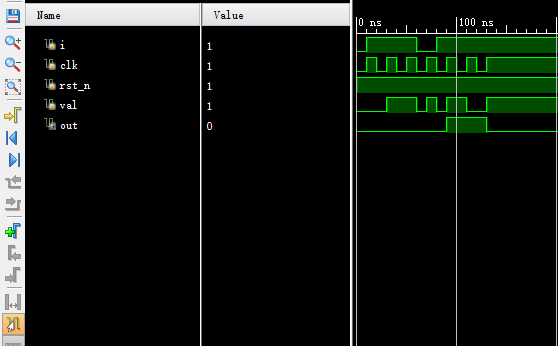
\includegraphics[width=1\textwidth]{fsm.png}
\end{figure}
\begin{figure}[H]
  \centering
  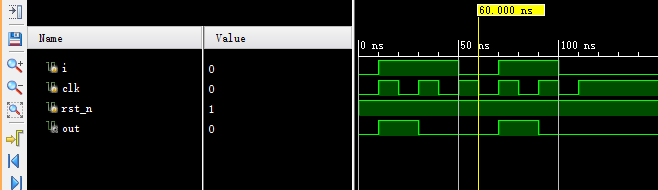
\includegraphics[width=1\textwidth]{remove_glitch.png}
\end{figure}
\section{实验分析}
\paragraph{1}一定得按要求来写,我最开始没有写三段式,所以后来重写了
\paragraph{2}由于抖动时间为5ms--10ms,所有要计算去毛刺的时钟周期数,我用的50mhz的,所以取了250000
\paragraph{3}先去毛刺,然后得到上升沿,这里也有一些技巧
\paragraph{4}实验仿真也不能拘泥,比如仿真时,要检查去毛刺模块,可以把时钟周期数改小

\section{源代码}

\begin{lstlisting}[language=verilog]
module top(
        input sw,bt,clk,rst_n,
        output  led
        );
        wire val;
        wire ol;
//        cnt ins(.in(bt),.clk(clk),.rst_n(rst_n),.ol(ol));
        remove_glitch  (.key_in(bt),.clk(clk),.key_out(ol));
        valid (.clk(clk),.rst_n(rst_n),.sig(ol),.out(val));
        state  (.clk(clk),.val(val),.rst_n(rst_n),.data(sw),.y(led));
endmodule


module cnt(
        input in,clk,rst_n,
        output reg ol
        );
        reg flag;
        reg [19:0]ct;
        initial begin ct=0; flag =0;ol=0; end
        always @(*)
            begin
                if(~rst_n) begin ol<=0; ct<=0; end 
                else
                   if(ct==250000) begin flag=0;ol=1;ct=0; end
                   else ol<=0;
                   if(flag) ct=ct+1;
                   else if(in)
                         begin flag=1;ct=ct+1 ; end
            end
endmodule


module valid(
    input clk,sig,rst_n,
    output reg out
    );
    reg flag;
    initial begin  flag =0;out=0;end
    always@(posedge clk,negedge rst_n)
        if(~rst_n) begin flag<=0; out<=0;  end
        else
        if(sig) 
            if(flag==1) out<=0;
            else begin out<=1; flag<=1; end
        else begin flag<=0; out<=0;end 
endmodule


module state(
    input rst_n,data,val,clk,
    output reg y
    );
    reg [1:0]st ;
    reg [1:0] last;
    parameter s0=2'b00,s1=2'b01,s2=2'b10,s3=2'b11;
    initial begin last=s0;y=0;  end
//    always @(posedge clk,negedge rst_n)
//        begin
//            if(~rst_n) begin st<=s0;y<=0; end
//            else 
//                if(val)
//                begin
//                case(st)
//                s0:begin    y<=0;if(data) st<=s1; end
//                s1:if(data) begin st<=s2; y<=0; end  
//                   else begin st<=s0; y<=0;  end
//                s2:if(~data) begin st<=s3; y<=0; end
//                s3:begin 
//                    st<=s0;
//                    if(data) y<=1;else y<=0;
//                   end
//                endcase
//                end
//        end
    always @(posedge clk,negedge rst_n)
        if(~rst_n) st<=s0;
        else st<=last;   
        
        
           
    always @(*)
    begin
        if(val)
        case(last)
            s0:if(data) last<=s1;
             s1:if(data) begin last<=s2; end  
                       else begin last<=s0;end
             s2:if(~data)  last<=s3; 
             s3:last<=s0;
             endcase
         end
         
         
       always@(*)   
               if(val&&st==2'b11&&data)y<=1;
               else y<=0;
endmodule
\end{lstlisting}


状态原理图
\begin{figure}[H]
  \centering
  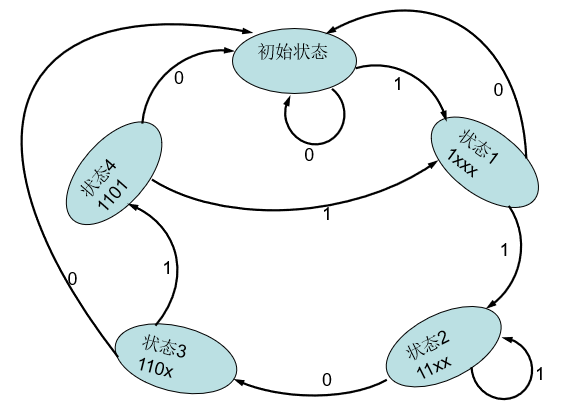
\includegraphics[width=1\textwidth]{states.png}
\end{figure}
\end{document}